% begin module limit-at-infinity-intro
\begin{frame}
\frametitle{Limits at Infinity; Horizontal Asymptotes}
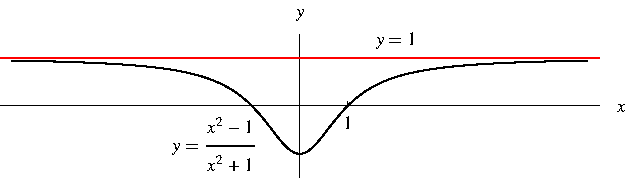
\includegraphics[width=12cm]{curve-sketching/pictures/04-04-intro.pdf}%
\begin{columns}[c]
\column{.3\textwidth}
\uncover<2->{%
\[
\begin{array}{|r|r@{}l|}
\hline
x & & \ \ f(x)\\
\hline
0 & - & 1\\
  \pm 1 &  & 0\\
  \pm 2 &  & 0.600000\\
  \pm 3 &  & 0.800000\\
  \pm 4 &  & 0.882353\\
  \pm 5 &  & 0.923077\\
 \pm 10 &  & 0.980198\\
%\pm 100 &  & 0.999800\\
\hline
\end{array}
\]
}%
\column{.7\textwidth}
\begin{itemize}
\item  Consider $f(x) = \frac{x^2-1}{x^2+1}$ as $x$ becomes large.
\item<2->  The values of $f(x)$ get closer and closer to $1$.
\item<3->  We express this by writing $\lim_{x\to \infty} f(x) = 1$.
\item<4->  When $x$ is large negative, $f(x)$ is also near $1$.
\item<5->  We express this by writing $\lim_{x\to -\infty} f(x) = 1$.
\end{itemize}
\end{columns}
\end{frame}
% end module limit-at-infinity-intro
